\documentclass[../thesis.tex]{subfiles}
\section{Hệ thống hoá Các chính sách Chương trình MTQG phát triển Nông thôn mới có liên quan tới không gian kiến trúc cảnh quan từ 2009-2020}
\subsection {Bối cảnh chính sách NTM dưới góc nhìn về QHXD}

\textit{Khởi nguồn:} Cụm từ NTM được nhắc tới lần đầu trong văn bản quy phạm pháp luật chính thức là trong Nghị quyết số 26-NQ/TW\cite{nq26nqtw}, ngày 05/8/2008, Hội nghị lần thứ Bảy Ban Chấp hành Trung ương Đảng (khóa X). Trên cơ sở những vấn đề về Vùng và Liên Vùng, bao gồm: hạn chế trong phát triển Nông nghiệp, quy mô sản xuất còn nhỏ lẻ và manh mún, sự yếu kém về quy hoạch hạ tầng, đời sống người dân còn khó khăn; Hội nghị đã đề ra các quan điểm liên quan tới phát triển NTM:
\begin{enumerate}
\item“ \textbf{Nông nghiệp, nông dân, nông thôn có vị trí chiến lược trong sự nghiệp công nghiệp hoá, hiện đại hoá, xây dựng và bảo vệ Tổ quốc}, là cơ sở và lực lượng quan trọng để phát triển kinh tế - xã hội bền vững, giữ vững ổn định chính trị, đảm bảo an ninh, quốc phòng; giữ gìn, phát huy bản sắc văn hoá dân tộc và bảo vệ môi trường sinh thái của đất nước.
\item \textbf{Các vấn đề nông nghiệp, nông dân, nông thôn phải được giải quyết đồng bộ, gắn với quá trình đẩy mạnh công nghiệp hoá, hiện đại hoá đất nước}. Công nghiệp hoá, hiện đại hoá nông nghiệp, nông thôn là một nhiệm vụ quan trọng hàng đầu của quá trình công nghiệp hoá, hiện đại hoá đất nước. Trong mối quan hệ mật thiết giữa nông nghiệp, nông dân và nông thôn, nông dân là chủ thể của quá trình phát triển, xây dựng nông thôn mới gắn với xây dựng các cơ sở công nghiệp, dịch vụ và phát triển đô thị theo quy hoạch là căn bản; phát triển toàn diện, hiện đại hóa nông nghiệp là then chốt.
\item \textbf{Phát triển nông nghiệp, nông thôn và nâng cao đời sống vật chất, tinh thần của nông dân phải dựa trên cơ chế kinh tế thị trường định hướng xã hội chủ nghĩa, phù hợp với điều kiện của từng vùng, từng lĩnh vực}, để giải phóng và sử dụng có hiệu quả các nguồn lực xã hội, trước hết là lao động, đất đai, rừng và biển; khai thác tốt các điều kiện thuận lợi trong hội nhập kinh tế quốc tế cho phát triển lực lượng sản xuất trong nông nghiệp, nông thôn; phát huy cao nội lực; đồng thời tăng mạnh đầu tư của Nhà nước và xã hội, ứng dụng nhanh các thành tựu khoa học, công nghệ tiên tiến cho nông nghiệp, nông thôn, phát triển nguồn nhân lực, nâng cao dân trí nông dân.
\item \textbf{Giải quyết vấn đề nông nghiệp, nông dân, nông thôn là nhiệm vụ của cả hệ thống chính trị và toàn xã hộ}i; trước hết, phải khơi dậy tinh thần yêu nước, tự chủ, tự lực tự cường vươn lên của nông dân. Xây dựng xã hội nông thôn ổn định, hoà thuận, dân chủ, có đời sống văn hóa phong phú, đàm đà bản sắc dân tộc, tạo động lực cho phát triển nông nghiệp và xây dựng nông thôn mới, nâng cao đời sống nông dân.”
\end{enumerate}
Theo quan điểm được nêu trên, \textit{Nông nghiệp, Nông dân và Nông thôn} (1) \textbf{có vai trò quan trọng trong thời đại mới},(2) là một \textbf{vấn đề cần được giải quyết đồng bộ},(3)\textbf{nâng cao chất lượng cuộc sống trên cơ sở từng khu vực, từng lĩnh vực}, và (4) là \textbf{trách nhiệm của hệ thống chính trị và xã hội}.
Từ những lý luận gốc của chương trình NTM, luận văn đặt vấn đề dưới góc nhìn lĩnh vực Kiến trúc- Xây dựng (biến đổi không gian kiến trúc cảnh quan) tại một khu vực cụ thể (xã Thụy Hương) nhằm đối chiếu với những tiêu chuẩn chung, đánh giá chất lượng phát triển không gian kiến trúc cảnh quan khu vực, cải thiện chất lượng cuộc sống người dân khu vực.


Việc phát triển NTM giai đoạn 2010-2020 có thể chia thành hai giai đoạn chính:
\begin{enumerate}
\item 2008 - 2015: Trong luận văn tạm gọi giai đoạn này là "giai đoạn 800" do được xác định bởi Quyết định số 800/QĐ-TTG \cite{qd800}
\item 2016 - 2020: Trong luận văn tạm gọi giai đoạn này là "giai đoạn 1600" do được xác định bởi Quyết định số 1600/QĐ-TTG \cite{qd800}
\end{enumerate}
\begin{document}

Theo \textbf{Quyết định số 800/QĐ-TTG \cite{qd800}} Chương trình NTM giai đoạn 2010-2020 được định hướng “Xây dựng nông thôn mới có kết cấu hạ tầng kinh tế - xã hội từng bước hiện đại; cơ cấu kinh tế và các hình thức tổ chức sản xuất hợp lý, gắn nông nghiệp với phát triển nhanh công nghiệp, dịch vụ; gắn phát triển nông thôn với đô thị theo quy hoạch; xã hội nông thôn dân chủ, ổn định, giàu bản sắc văn hóa dân tộc; môi trường sinh thái được bảo vệ; an ninh trật tự được giữ vững; đời sống vật chất và tinh thần của người dân ngày càng được nâng cao; theo định hướng xã hội chủ nghĩa”. Từ 2016, định hướng đặc trưng này được tái khẳng định “Xây dựng nông thôn mới để nâng cao đời sống vật chất và tinh thần cho người dân; có kết cấu hạ tầng kinh tế - xã hội phù hợp; cơ cấu kinh tế và các hình thức tổ chức sản xuất hợp lý, gắn phát triển nông nghiệp với công nghiệp, dịch vụ; gắn phát triển nông thôn với đô thị; xã hội nông thôn dân chủ, bình đẳng, ổn định, giàu bản sắc văn hóa dân tộc; môi trường sinh thái được bảo vệ; quốc phòng và an ninh, trật tự được giữ vững.”\textbf{ (Quyết định 1600/QĐ-TTg \cite{qd1600})}\\

Thông qua hai quyết định 800/QĐ-TTg và 1600/QĐ-TTG, có thể khái quát NTM là một chương trình phát triển những khu vực nông thôn nhằm bổ sung, \textit{(1)kết nối những hạ tầng cần thiết cho quá trình phát triển KT-XH,(2)nâng cao chất lượng đời sống người dân,(3) đưa phát triển nông thôn song hành cùng phát triển đô thị.}


\begin{tabular}{ | m{7.5cm} | m{7.5cm}| } 
\hline      
\multicolumn{1}{|c|}{\textbf{Quyết định số 800/QĐ-TTG}}& \multicolumn{1}{c|}{\textbf{Quyết định số 1600/QĐ-TTG}} \\
\hline  
“Xây dựng nông thôn mới có \textbf{kết cấu hạ tầng kinh tế - xã hội từng bước hiện đại}; cơ cấu kinh tế và các hình thức tổ chức sản xuất hợp lý, gắn nông nghiệp với phát triển nhanh công nghiệp, dịch vụ;\textbf{ gắn phát triển nông thôn với đô thị theo quy hoạch}; xã hội nông thôn dân chủ, ổn định, giàu bản sắc văn hóa dân tộc; môi trường sinh thái được bảo vệ; an ninh trật tự được giữ vững;\textbf{ đời sống vật chất và tinh thần của người dân ngày càng được nâng cao}; theo định hướng xã hội chủ nghĩa” & “Xây dựng nông thôn mới để \textbf{nâng cao đời sống vật chất và tinh thần cho người dân; có kết cấu hạ tầng kinh tế - xã hội phù hợp}; cơ cấu kinh tế và các hình thức tổ chức sản xuất hợp lý, gắn phát triển nông nghiệp với công nghiệp, dịch vụ; \textbf{gắn phát triển nông thôn với đô thị}; xã hội nông thôn dân chủ, bình đẳng, ổn định, giàu bản sắc văn hóa dân tộc; môi trường sinh thái được bảo vệ; quốc phòng và an ninh, trật tự được giữ vững.”\\
\hline 
\end{tabular} \\

\subsection {Khái quát hệ thống tiêu chí NTM}

Cụ thể hóa \textbf{Nghị quyết số 26-NQ TW Hội nghị Trung ương 7 khóa X} ,\textbf{ TT-CP} đã đưa ra\textbf{ QĐ 491 VỀ VIỆC BAN HÀNH BỘ TIÊU CHÍ QUỐC GIA VỀ NÔNG THÔN MỚI}
Quyết định này bao gồm 19 tiêu chí được nhóm thành 5 nhóm:
\begin{itemize}
\item I. Quy hoạch
\item II. Hạ tầng KT-XH
\item III. Kinh tế và tổ chức sản xuất
\item IV. Văn hóa - Xã hội - Môi trường
\item V. Hệ thống chính trị
\end{itemize}
Trên cơ sở BTCQGNTM (QĐ 491-TTG và 1980-TTG), tác giả phân tích các tiêu chí có ảnh hưởng tới không gian kiến trúc cảnh quan khu vực.
\begin{figure}[ht!]
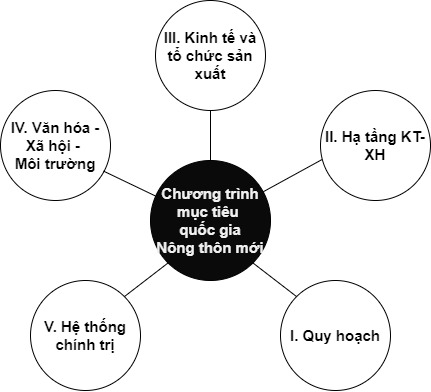
\includegraphics[width=10cm]{491_QĐ-TTg(1).jpg}
\caption{Cấu trúc BỘ TIÊU CHÍ QUỐC GIA VỀ NÔNG THÔN MỚI}
\end{figure}

\begin{landscape}
\begin{longtable}{|p{2cm}|p{2cm}|p{4cm}|p{2cm}|p{1cm}|p{1cm}|p{1cm}|p{1cm}|p{1cm}|p{1cm}|p{1cm}|}
\hline
\multicolumn{1}{|c|}{\multirow{2}{*}{\textbf{TT}}} &
  \multirow{2}{2cm}{Tên tiêu chí} &
  \multirow{2}{4cm}{Nội dung tiêu chí} &
  \multirow{2}{2cm}{Chỉ tiêu chung} &
  \multicolumn{7}{l|}{Chỉ tiêu theo vùng} \\ \cline{5-11} 
\multicolumn{1}{|c|}{} &
   &
   &
   &
  TDMN   phía Bắc &
  Đồng   bằng sông Hồng &
  Bắc   Trung bộ &
  Duyên   hải Nam TB &
  Tây   Nguyên &
  Đông   Nam bộ &
  ĐB   sông Cửu Long \\ \hline
\endfirsthead
%
\endhead
%
\multicolumn{1}{|c|}{\multirow{4}{*}{2}} &
  \multirow{4}{*}{Giao   thông} &
  2.1. Tỷ lệ km đường trục xã,   liên xã được nhựa hóa hoặc bê tông hóa đạt chuẩn theo cấp kỹ thuật của Bộ   GTVT &
  100\% &
  100\% &
  100\% &
  100\% &
  100\% &
  100\% &
  100\% &
  100\% \\ \cline{3-11} 
\multicolumn{1}{|c|}{} &
   &
  2.2. Tỷ lệ km đường trục thôn,   xóm được cứng hóa đạt chuẩn theo cấp kỹ thuật của Bộ GTVT &
  70\% &
  50\% &
  100\% &
  70\% &
  70\% &
  70\% &
  100\% &
  50\% \\ \cline{3-11} 
\multicolumn{1}{|c|}{} &
   &
  2.3. Tỷ lệ km đường ngõ, xóm sạch   và không lầy lội vào mùa mưa. &
  100\% &
  100\%   (50\% cứng hóa) &
  100\%   cứng hóa &
  100\%   (70\% cứng hóa) &
  100\%   (70\% cứng hóa) &
  100\%   (50\% cứng hóa) &
  100\%   cứng hóa &
  100\%   (30\% cứng hóa) \\ \cline{3-11} 
\multicolumn{1}{|c|}{} &
   &
  2.4. Tỷ lệ km đường trục chính   nội đồng được cứng hóa, xe cơ giới đi lại thuận tiện &
  65\% &
  50\% &
  100\% &
  70\% &
  70\% &
  70\% &
  100\% &
  50\% \\ \hline
\multirow{2}{*}{3} &
  \multirow{2}{*}{Thủy   lợi} &
  3.1. Hệ thống thủy lợi cơ bản   đáp ứng yêu cầu sản xuất và dân sinh &
  Đạt &
  Đạt &
  Đạt &
  Đạt &
  Đạt &
  Đạt &
  Đạt &
  Đạt \\ \cline{3-11} 
 &
   &
  3.2. Tỷ lệ km trên mương do xã   quản lý được kiên cố hóa &
  65\% &
  50\% &
  85\% &
  85\% &
  70\% &
  45\% &
  85\% &
  45\% \\ \hline
4 &
  Điện &
  4.1. Hệ thống điện đảm bảo yêu   cầu kỹ thuật của ngành điện &
  Đạt &
  Đạt &
  Đạt &
  Đạt &
  Đạt &
  Đạt &
  Đạt &
  Đạt \\ \cline{3-11} 
 &
   &
  4.2. Tỷ lệ hộ sử dụng điện thường   xuyên, an toàn từ các nguồn &
  98\% &
  95\% &
  99\% &
  98\% &
  98\% &
  98\% &
  99\% &
  98\% \\ \cline{3-11} 
5 &
  Trường   học &
  Tỷ lệ trường học các cấp: mầm   non, mẫu giáo, tiểu học, THCS có cơ sở vật chất đạt chuẩn quốc gia &
  80\% &
  70\% &
  100\% &
  80\% &
  80\% &
  70\% &
  100\% &
  70\% \\ \cline{3-11} 
\multirow{2}{*}{6} &
  \multirow{2}{*}{Cơ   sở vật chất văn hóa} &
  6.2. Nhà văn hóa và khu thể   thao xã đạt chuẩn của Bộ VH-TT-DL &
  Đạt &
  Đạt &
  Đạt &
  Đạt &
  Đạt &
  Đạt &
  Đạt &
  Đạt \\ \cline{3-11} 
 &
   &
  6.3. Tỷ lệ thôn có nhà văn hóa   và khu thể thao thôn đạt quy định của Bộ VH-TT-DL &
  100\% &
  100\% &
  100\% &
  100\% &
  100\% &
  100\% &
  100\% &
  100\% \\ \cline{3-11} 
7 &
  Chợ nông thôn &
  Chợ đạt chuẩn   của Bộ Xây dựng &
  Đạt &
  Đạt &
  Đạt &
  Đạt &
  Đạt &
  Đạt &
  Đạt &
  Đạt \\ \cline{3-11} 
\multirow{2}{*}{8} &
  \multirow{2}{2cm}{Bưu   điện} &
  8.1. Có điểm phục vụ bưu chính   viễn thông. &
  Đạt &
  Đạt &
  Đạt &
  Đạt &
  Đạt &
  Đạt &
  Đạt &
  Đạt \\ \cline{3-11} 
 &
   &
  8.2. Có Internet đến thôn &
  Đạt &
  Đạt &
  Đạt &
  Đạt &
  Đạt &
  Đạt &
  Đạt &
  Đạt \\ \cline{3-11} 
\multirow{2}{*}{9} &
  \multirow{2}{2cm}{Nhà   ở dân cư} &
  9.1. Nhà tạm, dột nát &
  Không &
  Không &
  Không &
  Không &
  Không &
  Không &
  Không &
  Không \\ \cline{3-11} 
 &
   &
  9.2. Tỷ lệ hộ có nhà ở đạt   tiêu chuẩn Bộ Xây dựng &
  80\% &
  75\% &
  90\% &
  80\% &
  80\% &
  75\% &
  90\% &
  70\% \\ 
  \hline
\end{longtable}
\textit{Kinh tế và tổ chức sản xuất}
\begin{longtable}{|p{2cm}|p{2cm}|p{4cm}|p{2cm}|p{1cm}|p{1cm}|p{1cm}|p{1cm}|p{1cm}|p{1cm}|p{1cm}|}
\hline
\multicolumn{1}{|c|}{\multirow{2}{*}{\textbf{TT}}} &
  \multirow{2}{2cm}{Tên tiêu chí} &
  \multirow{2}{4cm}{Nội dung tiêu chí} &
  \multirow{2}{2cm}{Chỉ tiêu chung} &
  \multicolumn{7}{l|}{Chỉ tiêu theo vùng} \\ \cline{5-11} 
\multicolumn{1}{|c|}{} &
   &
   &
   &
  TDMN   phía Bắc &
  Đồng   bằng sông Hồng &
  Bắc   Trung bộ &
  Duyên   hải Nam TB &
  Tây   Nguyên &
  Đông   Nam bộ &
  ĐB   sông Cửu Long \\ \hline
\endfirsthead
%
\endhead
%
\multicolumn{1}{|c|}{10} &
  Thu   nhập &
  Thu nhập   bình quân đầu người/năm so với mức bình quân chung của tỉnh &
  1,4 lần &
  1,2 lần &
  1,5 lần &
  1,4 lần &
  1,4   lần &
  1,3 lần &
  1,5 lần &
  1,3   lần \\ \hline
11 &
  Hộ   nghèo &
  Tỷ lệ hộ nghèo &
  \textless   6\% &
  10\% &
  3\% &
  5\% &
  5\% &
  7\% &
  3\% &
  7\% \\ \hline
12 &
  Cơ cấu lao động &
  Tỷ lệ lao động   trong độ tuổi làm việc trong lĩnh vực nông, lâm, ngư nghiệp &
  \textless 30\% &
  45\% &
  25\% &
  35\% &
  35\% &
  40\% &
  20\% &
  35\% \\ \hline
13 &
  Hình   thức tổ chức sản xuất &
  Có tổ hợp tác hoặc hợp tác xã   hoạt động có hiệu quả &
  Có &
  Có &
  Có &
  Có &
  Có &
  Có &
  Có &
  Có \\ \hline
\end{longtable}
\textit{IV. Văn hóa - Xã hội - Môi trường}
\begin{longtable}{|p{2cm}|p{2cm}|p{4cm}|p{2cm}|p{1cm}|p{1cm}|p{1cm}|p{1cm}|p{1cm}|p{1cm}|p{1cm}|}
\hline
\multicolumn{1}{|c|}{\multirow{2}{*}{\textbf{TT}}} &
  \multirow{2}{2cm}{Tên tiêu chí} &
  \multirow{2}{4cm}{Nội dung tiêu chí} &
  \multirow{2}{2cm}{Chỉ tiêu chung} &
  \multicolumn{7}{l|}{Chỉ tiêu theo vùng} \\ \cline{5-11} 
\multicolumn{1}{|c|}{} &
   &
   &
   &
  TDMN   phía Bắc &
  Đồng   bằng sông Hồng &
  Bắc   Trung bộ &
  Duyên   hải Nam TB &
  Tây   Nguyên &
  Đông   Nam bộ &
  ĐB   sông Cửu Long \\ \hline
\endfirsthead
%
\endhead
%
\multicolumn{1}{|c|}{\multirow{3}{*}{14}} &
  \multirow{3}{*}{Giáo dục} &
  14.1. Phổ cập   giáo dục trung học &
  Đạt &
  Đạt &
  Đạt &
  Đạt &
  Đạt &
  Đạt &
  Đạt &
  Đạt \\ \cline{3-11} 
\multicolumn{1}{|c|}{} &
   &
  14.2. Tỷ lệ học sinh tốt nghiệp   THCS được tiếp tục học trung học (phổ thông, bổ túc, học nghề) &
  85\% &
  70\% &
  90\% &
  85\% &
  85\% &
  70\% &
  90\% &
  80\% \\ \cline{3-11} 
\multicolumn{1}{|c|}{} &
   &
  14.3. Tỷ lệ lao động qua đào tạo &
  \textgreater   35\% &
  \textgreater   20\% &
  \textgreater   40 \% &
  \textgreater   35\% &
  \textgreater   35\% &
  \textgreater   20\% &
  \textgreater   40\% &
  \textgreater   20\% \\ \hline
\multirow{2}{*}{15} &
  \multirow{2}{*}{Y tế} &
  15.1. Tỷ lệ   người dân tham gia các hình thức bảo hiểm y tế &
  30\% &
  20\% &
  40\% &
  30\% &
  30\% &
  20\% &
  40\% &
  20\% \\ \cline{3-11} 
 &
   &
  15.2. Y tế xã đạt chuẩn quốc   gia &
  Đạt &
  Đạt &
  Đạt &
  Đạt &
  Đạt &
  Đạt &
  Đạt &
  Đạt \\ \hline
16 &
  Văn   hóa &
  Xã có từ 70\% số thôn, bản trở   lên đạt tiêu chuẩn làng văn hóa theo quy định của Bộ VH-TT-DL &
  Đạt &
  Đạt &
  Đạt &
  Đạt &
  Đạt &
  Đạt &
  Đạt &
  Đạt \\ \hline
\multirow{5}{*}{17} &
  \multirow{5}{*}{Môi   trường} &
  17.1. Tỷ lệ hộ được sử dụng nước   sạch hợp vệ sinh theo quy chuẩn Quốc gia &
  85\% &
  70\% &
  90\% &
  85\% &
  85\% &
  85\% &
  90\% &
  75\% \\ \cline{3-11} 
 &
   &
  17.2. Các cơ sở SX-KD đạt tiêu   chuẩn về môi trường &
  Đạt &
  Đạt &
  Đạt &
  Đạt &
  Đạt &
  Đạt &
  Đạt &
  Đạt \\ \cline{3-11} 
 &
   &
  17.3. Không có các hoạt động   suy giảm môi trường và có các hoạt động phát triển môi trường xanh, sạch, đẹp &
  Đạt &
  Đạt &
  Đạt &
  Đạt &
  Đạt &
  Đạt &
  Đạt &
  Đạt \\ \cline{3-11} 
 &
   &
  17.4. Nghĩa trang được xây dựng   theo quy hoạch &
  Đạt &
  Đạt &
  Đạt &
  Đạt &
  Đạt &
  Đạt &
  Đạt &
  Đạt \\ \cline{3-11} 
 &
   &
  17.5. Chất thải, nước thải được   thu gom và xử lý theo quy định &
  Đạt &
  Đạt &
  Đạt &
  Đạt &
  Đạt &
  Đạt &
  Đạt &
  Đạt \\ \hline
\end{longtable}
\clearpage
\textit{V. Hệ thống chính trị}
\begin{longtable}{|p{2cm}|p{2cm}|p{4cm}|p{2cm}|p{1cm}|p{1cm}|p{1cm}|p{1cm}|p{1cm}|p{1cm}|p{1cm}|}
\hline
\multicolumn{1}{|c|}{\multirow{2}{*}{\textbf{TT}}} &
  \multirow{2}{2cm}{Tên tiêu chí} &
  \multirow{2}{4cm}{Nội dung tiêu chí} &
  \multirow{2}{2cm}{Chỉ tiêu chung} &
  \multicolumn{7}{l|}{Chỉ tiêu theo vùng} \\ \cline{5-11} 
\multicolumn{1}{|c|}{} &
   &
   &
   &
  TDMN   phía Bắc &
  Đồng   bằng sông Hồng &
  Bắc   Trung bộ &
  Duyên   hải Nam TB &
  Tây   Nguyên &
  Đông   Nam bộ &
  ĐB   sông Cửu Long \\ \hline
\endfirsthead
%
\endhead
%
\multirow{4}{*}{18} &
  \multirow{4}{2cm}{Hệ thống tổ chức chính trị  xã hội vững mạnh} &
  18.1. Cán bộ xã đạt chuẩn &
  Đạt &
  Đạt &
  Đạt &
  Đạt &
  Đạt &
  Đạt &
  Đạt &
  Đạt \\ \cline{3-11} 
 &
   &
  18.2. Có đủ các tổ chức trong   hệ thống chính trị cơ sở theo quy định. &
  Đạt &
  Đạt &
  Đạt &
  Đạt &
  Đạt &
  Đạt &
  Đạt &
  Đạt \\ \cline{3-11} 
 &
   &
  18.3. Đảng bộ, chính quyền xã   đạt tiêu chuẩn “trong sạch, vững mạnh” &
  Đạt &
  Đạt &
  Đạt &
  Đạt &
  Đạt &
  Đạt &
  Đạt &
  Đạt \\ \cline{3-11} 
 &
   &
  18.4. Các tổ chức đoàn thể   chính trị của xã đều đạt danh hiệu tiên tiến trở lên &
  Đạt &
  Đạt &
  Đạt &
  Đạt &
  Đạt &
  Đạt &
  Đạt &
  Đạt \\ \hline
19 &
  An   ninh, trật tự xã hội &
  An ninh, trật tự xã hội được   giữ vững &
  Đạt &
  Đạt &
  Đạt &
  Đạt &
  Đạt &
  Đạt &
  Đạt &
  Đạt \\ \hline
\end{longtable}
\end{landscape}
\begin{landscape}
\begin{figure}[ht!]
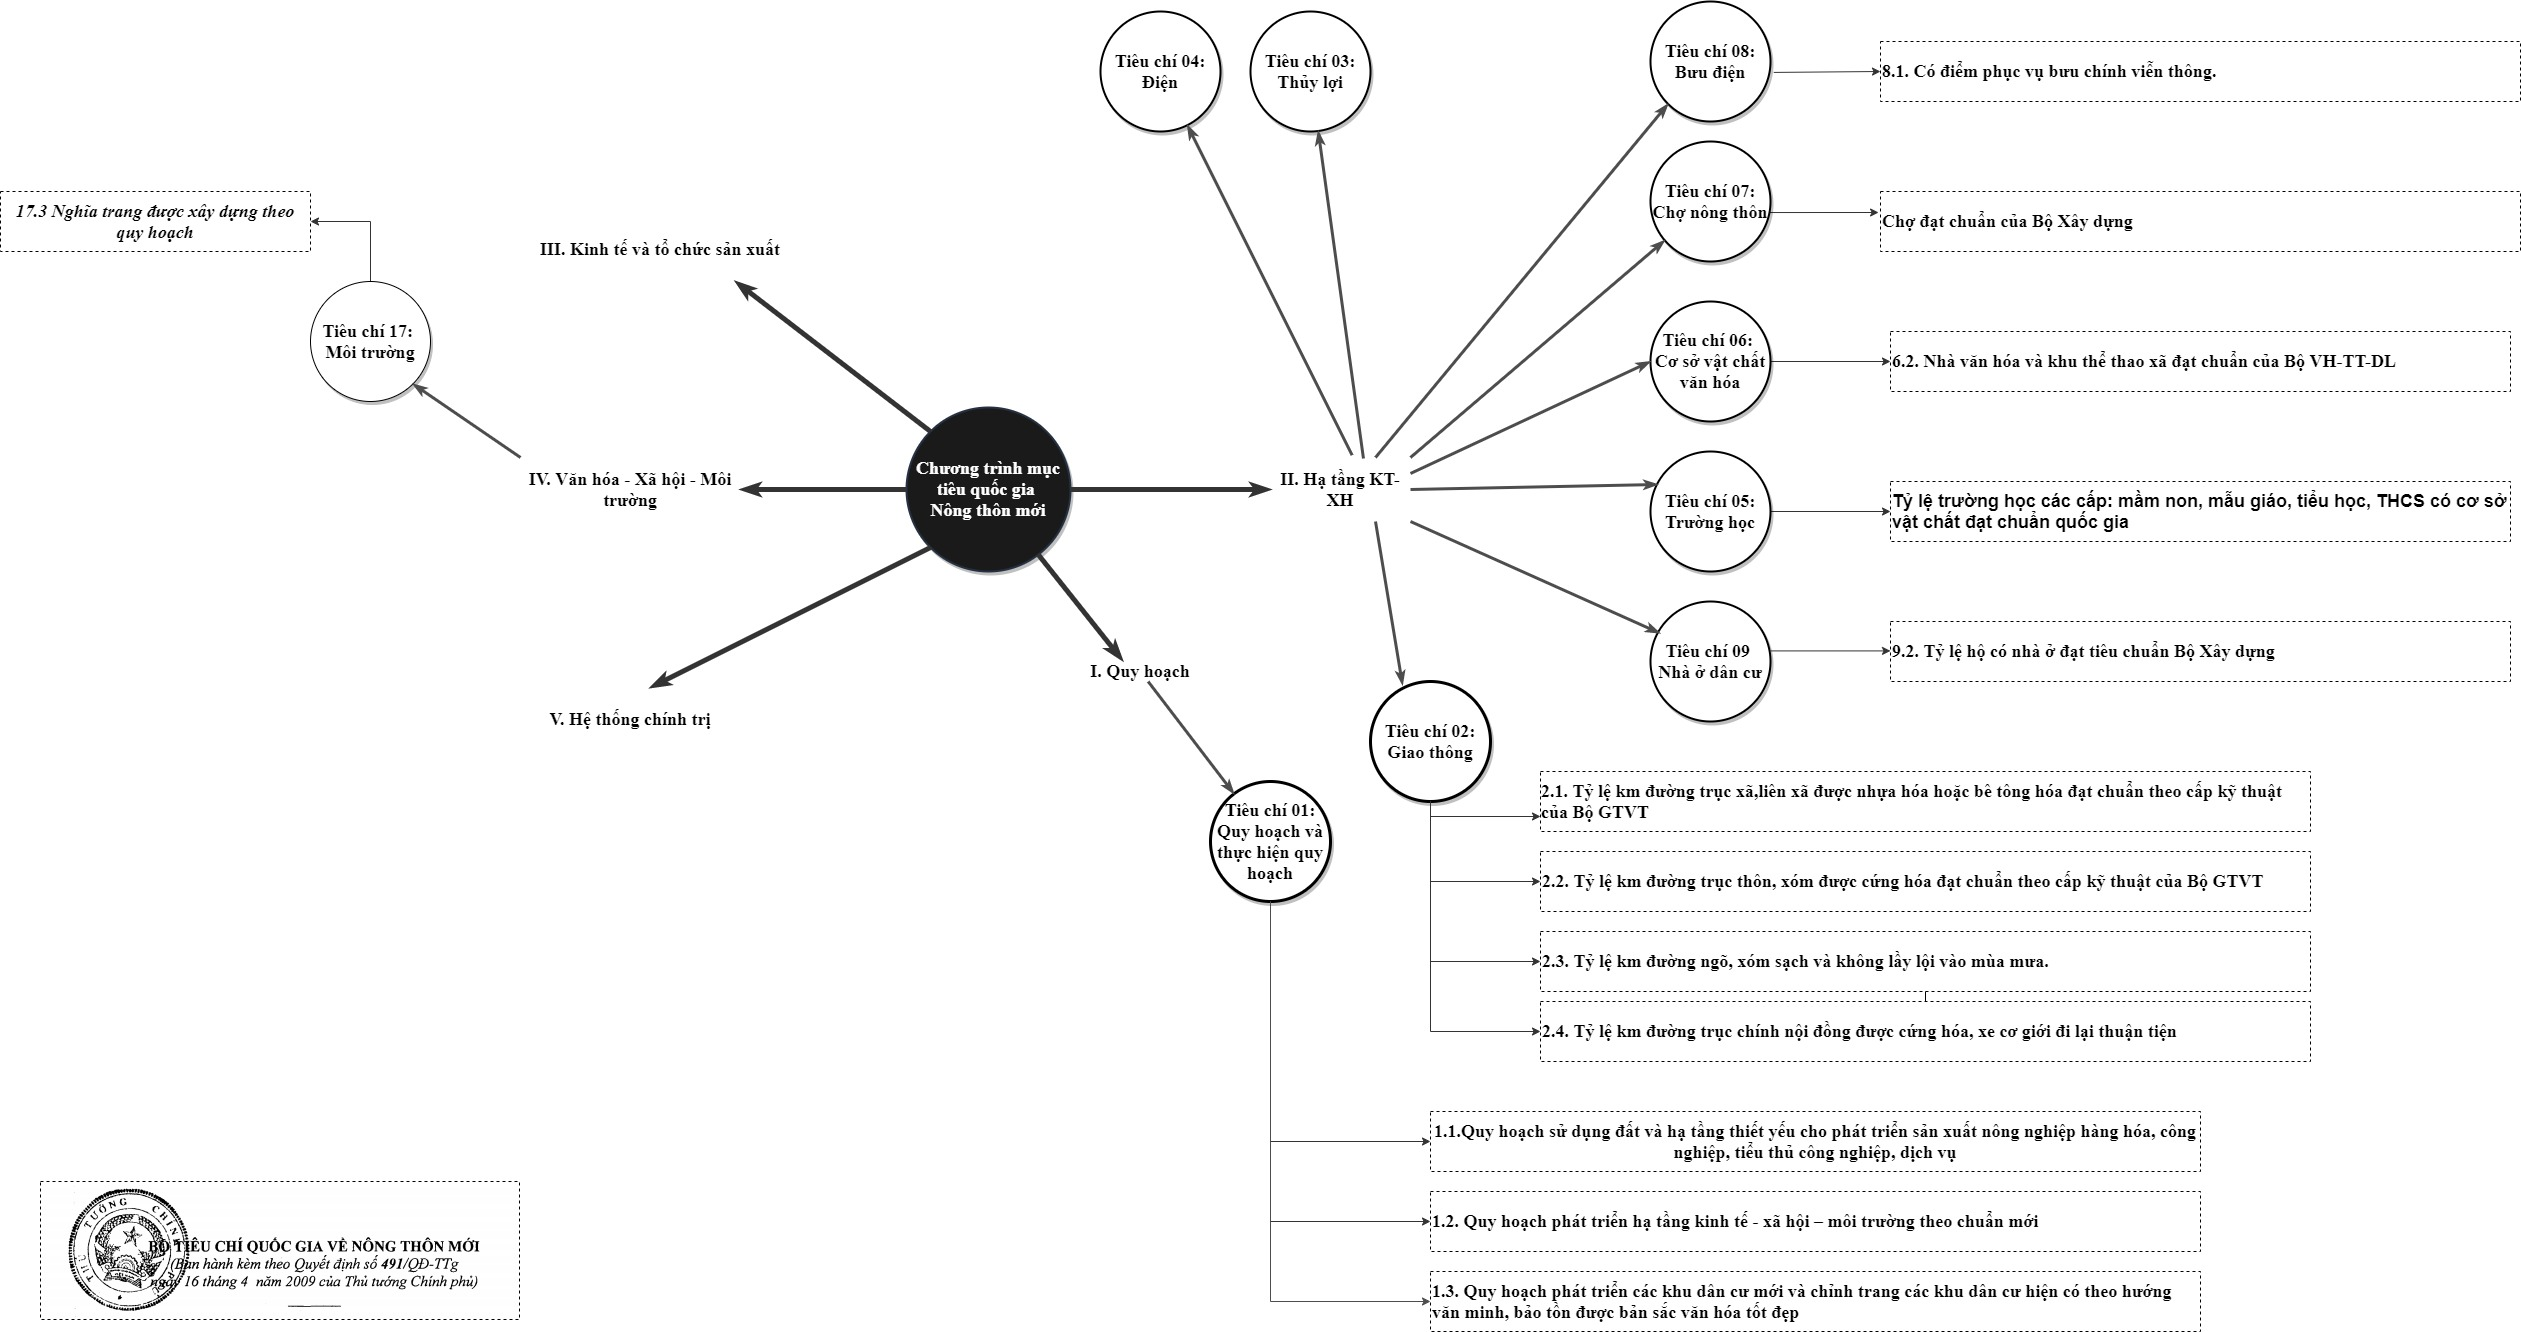
\includegraphics[width=24cm]{Graphic/491_QĐ-TTg.jpg}
\caption{Các tiêu chí ảnh hưởng tới KGKTCQ theo BTCQGNTM năm 2009}
\end{figure}
\clearpage

\begin{figure}[ht!]
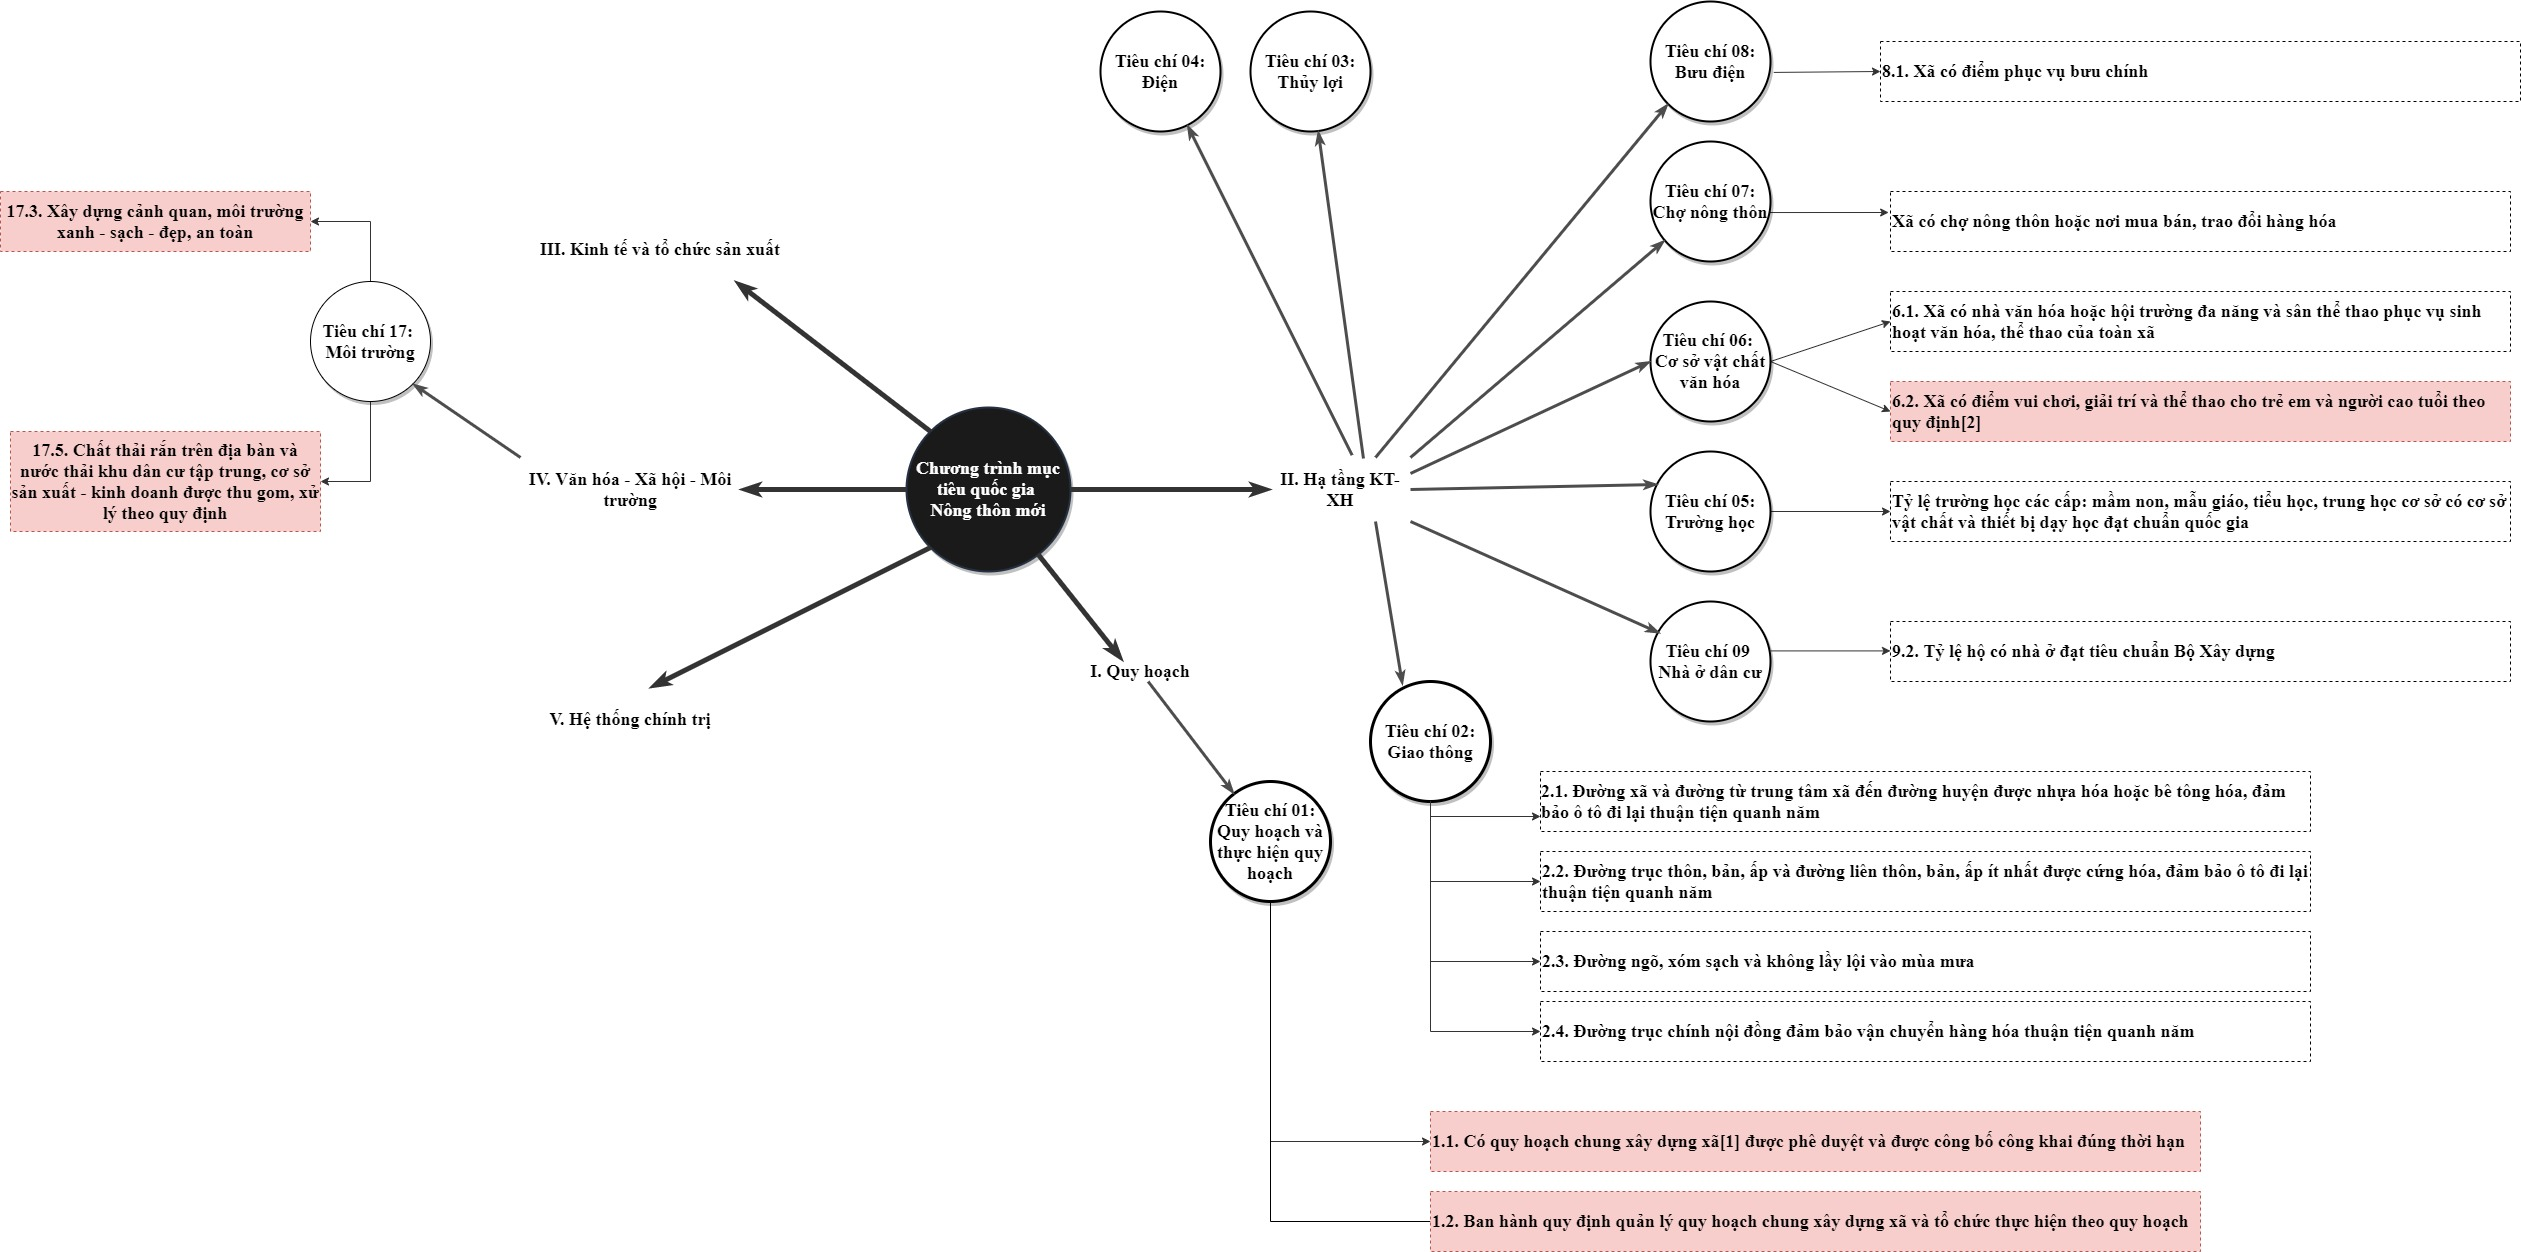
\includegraphics[width=24cm]{1980.jpg}
\caption{Các tiêu chí ảnh hưởng tới KGKTCQ theo BTCQGNTM giai đoạn 2016-2020}
\end{figure}

\end{landscape}
\textbf{Kết luận:} Các tiêu chí ảnh hưởng chính tới phát triển KGKTCQ trong CTMTQGNTM tập trung  tại nhóm I. Quy hoạch, II. Hạ tầng KT-XH và một tiêu chí thuộc nhóm IV.Văn hóa - Xã hội - Môi trường.

\section{Lý do lựa chọn khu vực nghiên cứu}
\subsection {Vị trí và mối liên hệ khu vực}
Xã Thuỵ Hương nằm ở phía Đông Huyện Chương Mỹ( Tây Thành phố Hà Nội), tiếp giáp:
\begin{itemize}
    \item Thị trấn Chúc Sơn ở phía Bắc
    \item Sông Đáy, Huyện Thanh Oai tại phía
    \item Xã Đại Yên ở phía Tây
    \item Xã Lam Điền ở phía Nam 
\end{itemize}
\begin{figure}[ht!]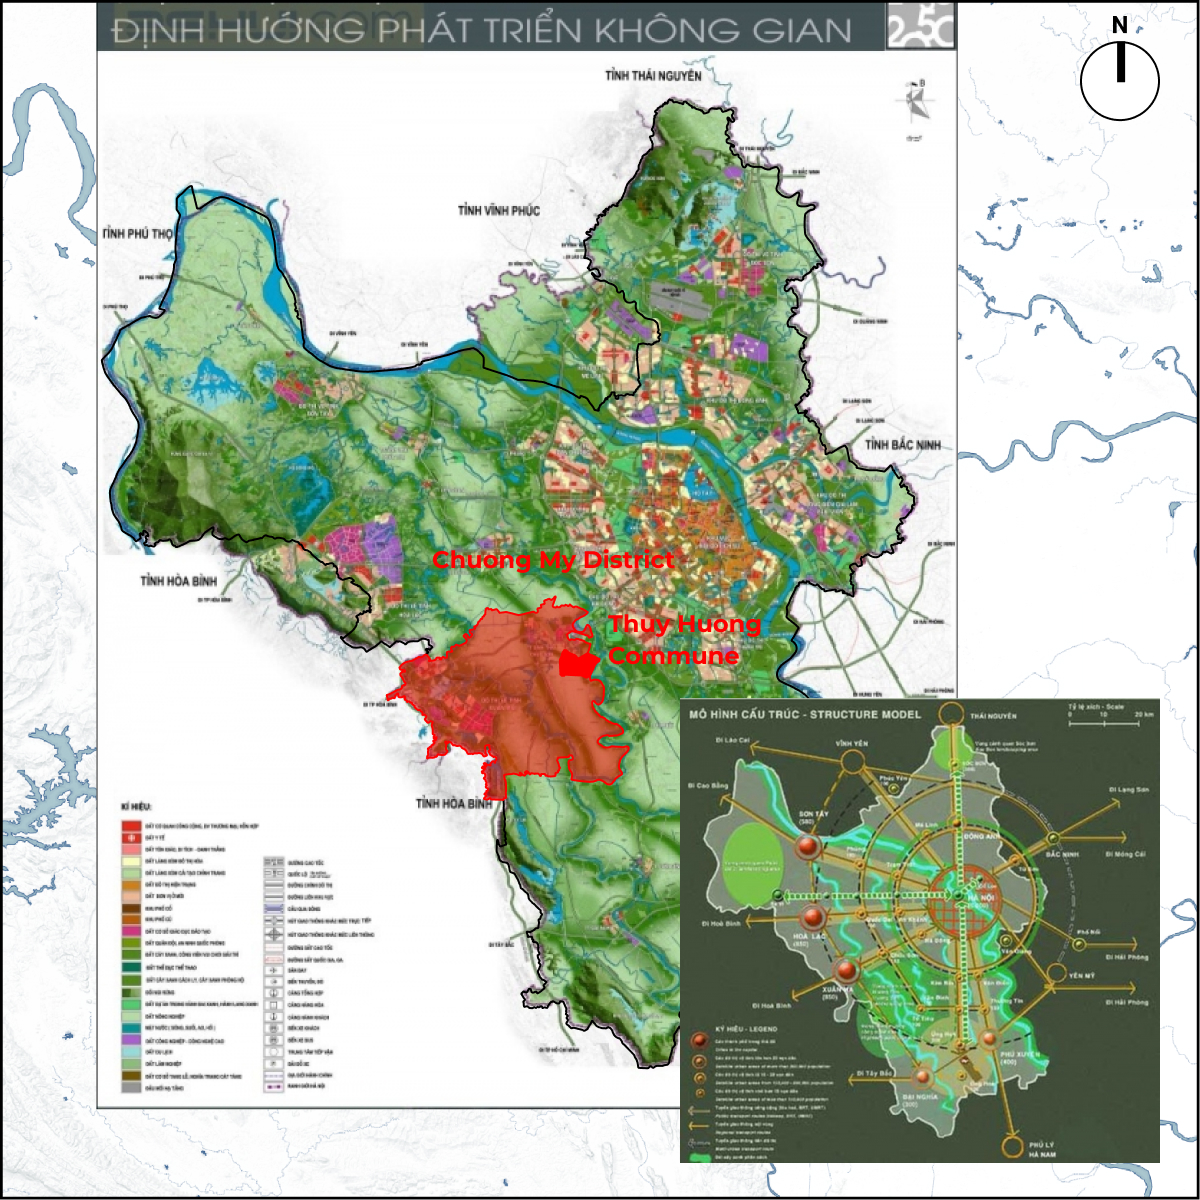
\includegraphics[width=10cm]{Vitri-TP.jpg}\caption{Vị trí xã Thụy Hương trong TP. Hà Nội}\end{figure}
Trong Quy hoạch chung Thành phố Hà Nội, khu vực xã Thuỵ Hương nằm trong\textbf{ vành đai sinh thái gắn liền với sông Đáy, vành đai liên kết các đô thị Chúc Sơn, Đông Anh.}
\begin{figure}[ht!]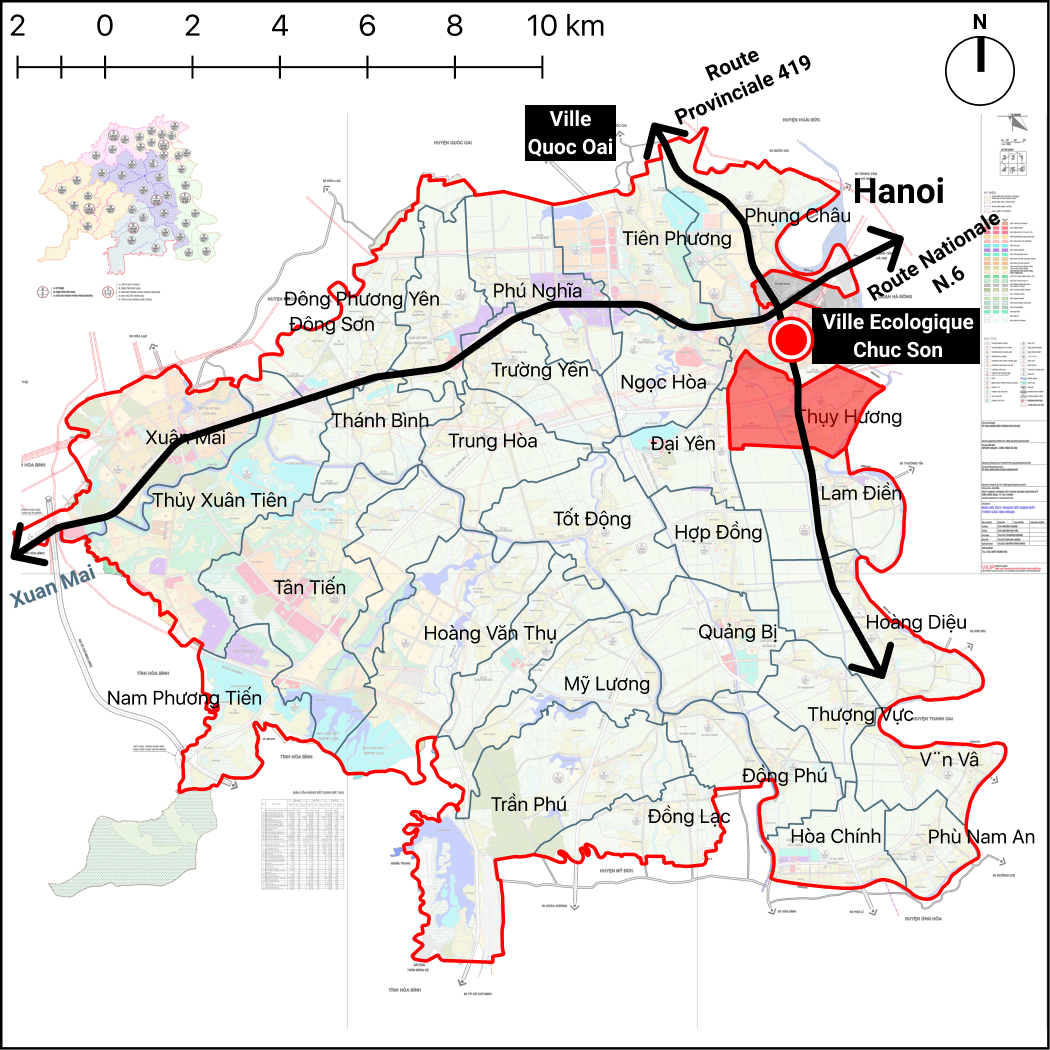
\includegraphics[width=10cm]{Graphic/Vitri-Huyen.jpg}\caption{Vị trí xã Thụy Hương trong Huyện Chương Mỹ}\end{figure}
Trong huyện Chương Mỹ, Xã Thuỵ Hương nằm ở phía Đông Bắc,gần hai tuyến đường quan trọng là đường (đê) Hữu Đáy - tỉnh lộ 419 song song với QL 21A và sông Đáy, đi qua TT. Quốc Oai, TT. Chúc Sơn.

\subsection {Tổng quan điều kiện tự nhiên}
Là vùng bãi ven sông Đáy, địa hình tương đối bằng phẳng thấp dần về phía Đông Nam. Chiều dài Đông - Tây 3 km và Bắc - Nam 2,1 km.\\
Khí hậu nhiệt đới gió mùa, nhiệt độ cao nhất 38- 400C (tháng 6 - 7), thấp nhất 4 - 60C (tháng 01- 02). Lượng mưa trung bình năm 1.600 - 1.800 mm.

\subsection {Cấu trúc không gian kiến trúc cảnh quan}

\begin{figure}
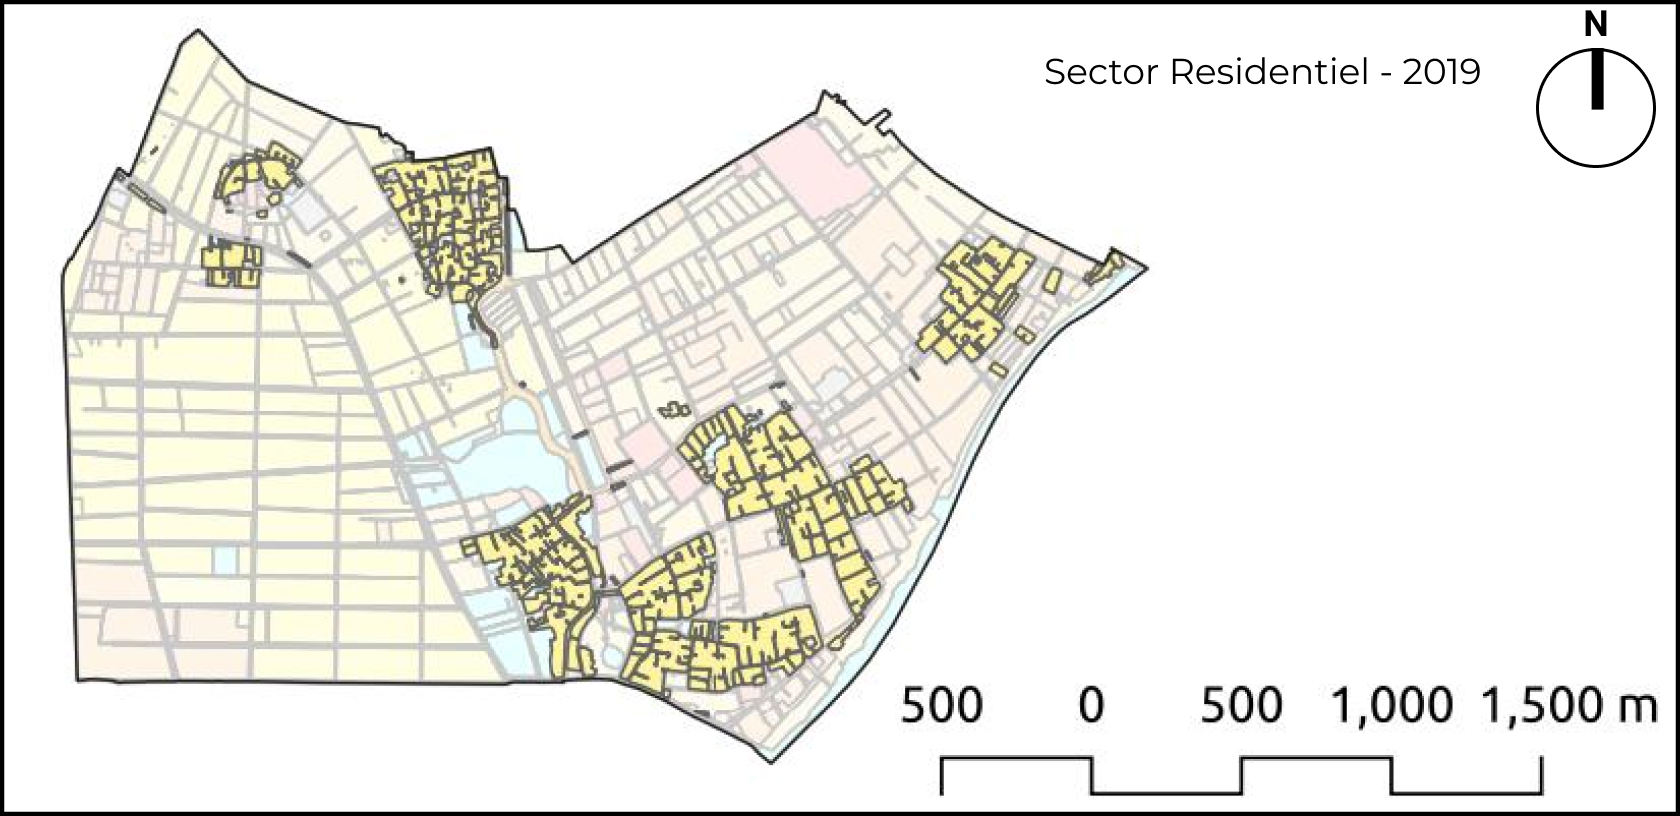
\includegraphics[width=15cm]{Graphic/spatial-structure.jpg}
\caption{Cấu trúc không gian các thôn xóm trong xã Thụy Hương}
\end{figure}


So với những làng ven sông dạng tuyến, cấu trúc không gian làng ở xã Thuỵ Hương có phần chặt chẽ về tổ chức không gian hơn. Không gian phân bố thành các khu vực rõ ràng, 
Mạng lưới đường giao thông phân bố đều, chia thành những cụm dân cư có diện tích giao động từ 0.2 - 2 ha. 

\subsection {Tổng quan kinh tế-xã hội khu vực nghiên cứu}
Trong Quyết định \textbf{“Về Việc Phê Duyệt Quy Hoạch Chung Xây Dựng Huyện Chương Mỹ Đến Năm 2030” Số: 2512/QĐ-UBND}, xã Thuỵ Hương thuộc hệ thống \textbf{“Vùng bãi"} với chức năng hỗ trợ sản xuất, chế biến rau an toàn, cụ thể : 
\quote{“Vùng bãi (bao gồm 7 xã: Thụy Hương, Lam Điền, Hoàng Diệu, Thượng Vực, Văn Võ, Phú Nam An, Hòa Chính) có diện tích khoảng 3.836,31 ha, dân số dự kiến năm 2030: 63.800 người. Hình thành Cụm đổi mới Hòa Chính là trung tâm xã Hòa Chính, tính chất chủ yếu hỗ trợ sản xuất vùng trồng rau an toàn, dịch vụ thương mại đầu mối và dịch vụ công cộng. Diện tích khoảng 20 - 25ha. Hỗ trợ mặt bằng sản xuất, chế biến rau an toàn, chuyển giao công nghệ, dịch vụ công cộng cho dân cư và gắn kết phát triển với khu dân cư hiện hữu xã Hòa Chính.”}\\

Theo số liệu 2009, thực trạng về nhân khẩu và lao động tại xã Thuỵ Hương:
\begin{itemize}
    \item Dân số xã Thụy Hương tính đến hết 2016 là: 8.062 người
    \item Mật độ dân số khu vực tính đến năm 2016 là 1470 người/km2

Theo DA2009, Lao động phân theo ngành nghề: nông nghiệp 2.039 (46,8\%); công nghiệp - tiểu thủ công nghiệp - xây dựng 1.480 (34\%); thương mại - dịch vụ - hành chính sự nghiệp 835 (19,2\%).

\end{itemize}
Mật độ dân số 
Lao động phân theo ngành nghề: nông nghiệp 2.039 (46,8\%); công nghiệp - tiểu thủ công nghiệp - xây dựng 1.480 (34\%); thương mại - dịch vụ - hành chính sự nghiệp 835 (19,2\%).

\subsection{Tổng quan về di sản khu vực}:
Một trong những di sản tiêu biểu của xã Thụy Hương là đình Thụy Dương
\quote{Đình Thụy Dương thôn Chúc Đồng thờ 6 vị thần Hoàng làng là : Thái Đường Đông Hải, Linh Lang Uy Sơn, Tam Tinh Tam Tê, Trình Lý Cha , Trình lý con và cao quyền công chúa. Đình có kiến trúc chữ Đinh với các hạng mục: đại bái và hậu cung. Đại bái gồm 5 gian hai trái kiểu 4 mái đao. Hậu cung là một nếp nhà ba gian , mái lợp ngói mũi hài. Đặc biệt đình còn lưu giữ được hệ thống hoành phi, cuốn thư, cửa võng trong di tích được chạm khắc tinh sảo, sơn son thếp vàng lộng lẫy .\footnote{Theo https://chuongmy.hanoi.gov.vn/}}

\subsection{Kết luận}
Có thể thấy xã Thụy Hương là một xã ven sông, nằm trên trục liên kết các Vệ Tinh thành phố Hà Nội, mât độ dân cư ở mức trung bình so với mật độ dân cư nông thôn thành phố Hà Nội, lao động địa phương chủ yếu là nông nghiệp và công nghiệp, có di sản, được định hướng phát triển trở thành một vùng trồng rau an toàn. Đya là một hình ảnh về một xã nông thôn cơ bản tại Thành phố Hà Nội.

\subsection {Cấu trúc không gian kiến trúc cảnh quan}

\begin{figure}
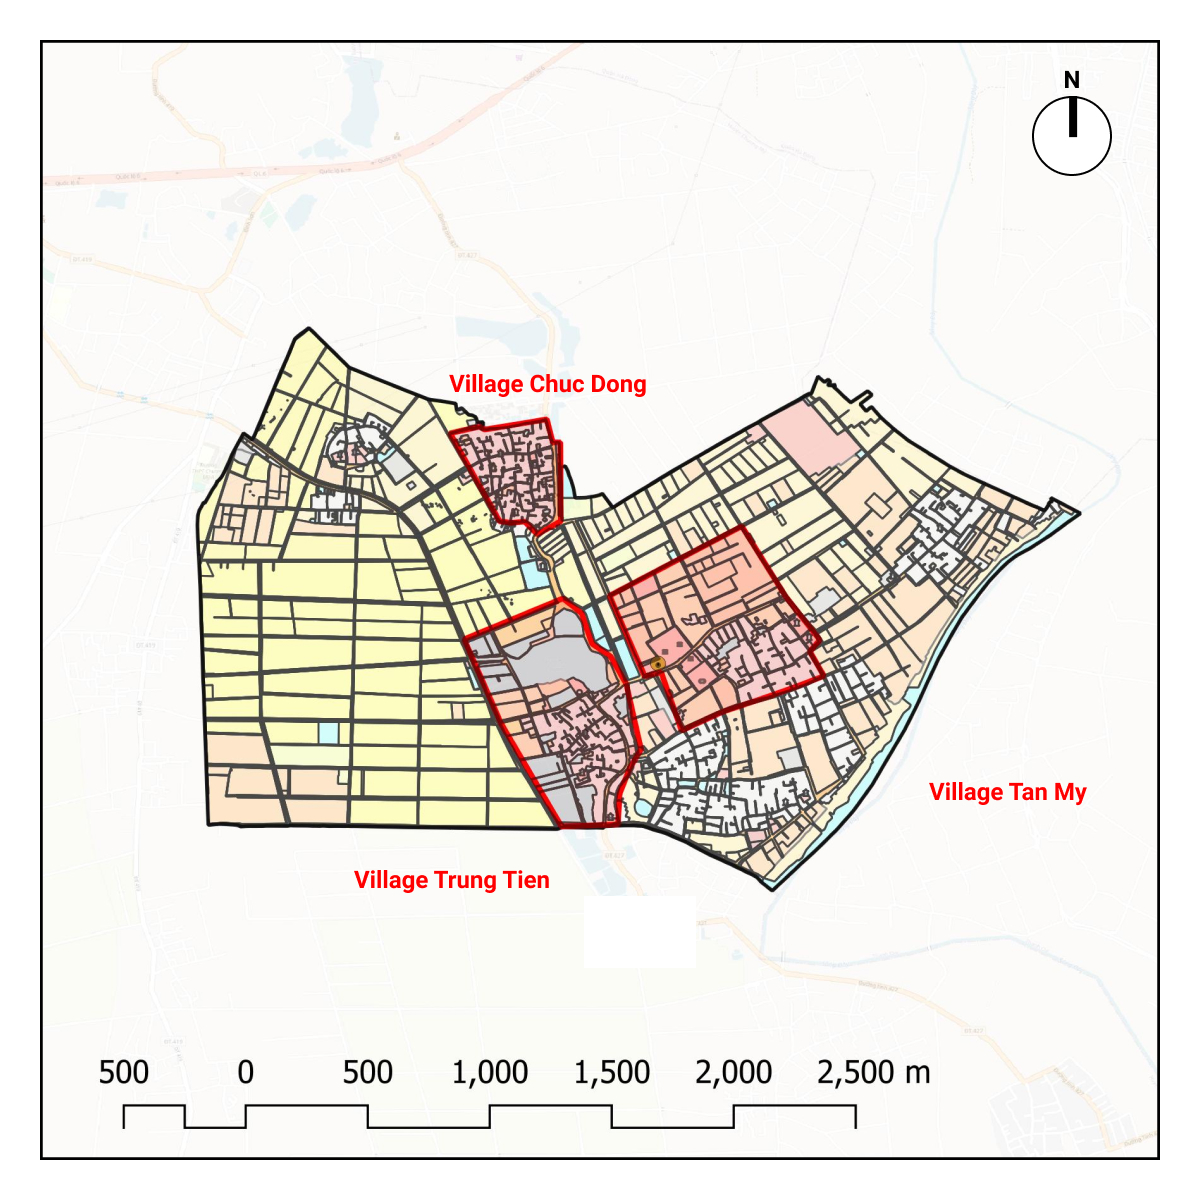
\includegraphics[width=15cm]{Graphic/Select.jpg}
\caption{Vị trí 3 thôn được lựa chọn}
\end{figure}



Trong nghiên cứu, luận văn tập trung nghiên cứu chi tiết 3 thôn Chúc Đồng, Trung Tiến và Phú Điền với lý do:
\begin{enumerate}
    \item Theo phân loại của học giả N.V.Huy (2019), ba thôn thuộc dạng làng thuần nông ven sông dạng tuyến - một dạng làng phổ biến ở vùng ĐBCTSH.
    \item Ba thôn được lựa chọn gần các trục giao thông chính,khu trung tâm nên hạ tầng được đầu tư tập trung hơn so với những thôn ở xa trung tâm, có thể nhận biết những biến động thông qua các bản quy hoạch
    \item Ba thôn có những vai trò nhất định trong xã: Thông Trung Tiến là khu trung tâm của xã, thôn Chúc Đồng tiếp giáp với TT. Sinh Thái Chúc Sơn nên có thể chịu ảnh hưởng đô thị hóa, thôn Phú Điền nằm trong khu vực phát triển HTX.
\end{enumerate}






\subsection {Tổng quan tình hình thực hiện NTM tại khu vực nghiên cứu}
\section {Kết luận chương}
	
\end{document}

